%\usepackage[normalem]{ulem}
%\useunder{\uline}{\ul}{}

\section{Results}

%This section should include the following:
%
%\begin{itemize}
%
%	
%	\item Details and explanations of results obtained (which itself could have
%		sub-sections). This is where you should provide tables, graphs, and/or
%		figures that illustrate your results. If you have created a new
%		application, include screenshots of it in action. You should also provide a
%		link to your application if it is web-based.
%
%\end{itemize}
%
%You should entitle these sections and sub-sections with names that describe the
%key points (for example, instead of ``methods we use", the heading
%``Statistical-Based Learning" would be more informative). The Methods and
%Results sections should together be approximately 3-4 pages in length.


\begin{figure}[H]
  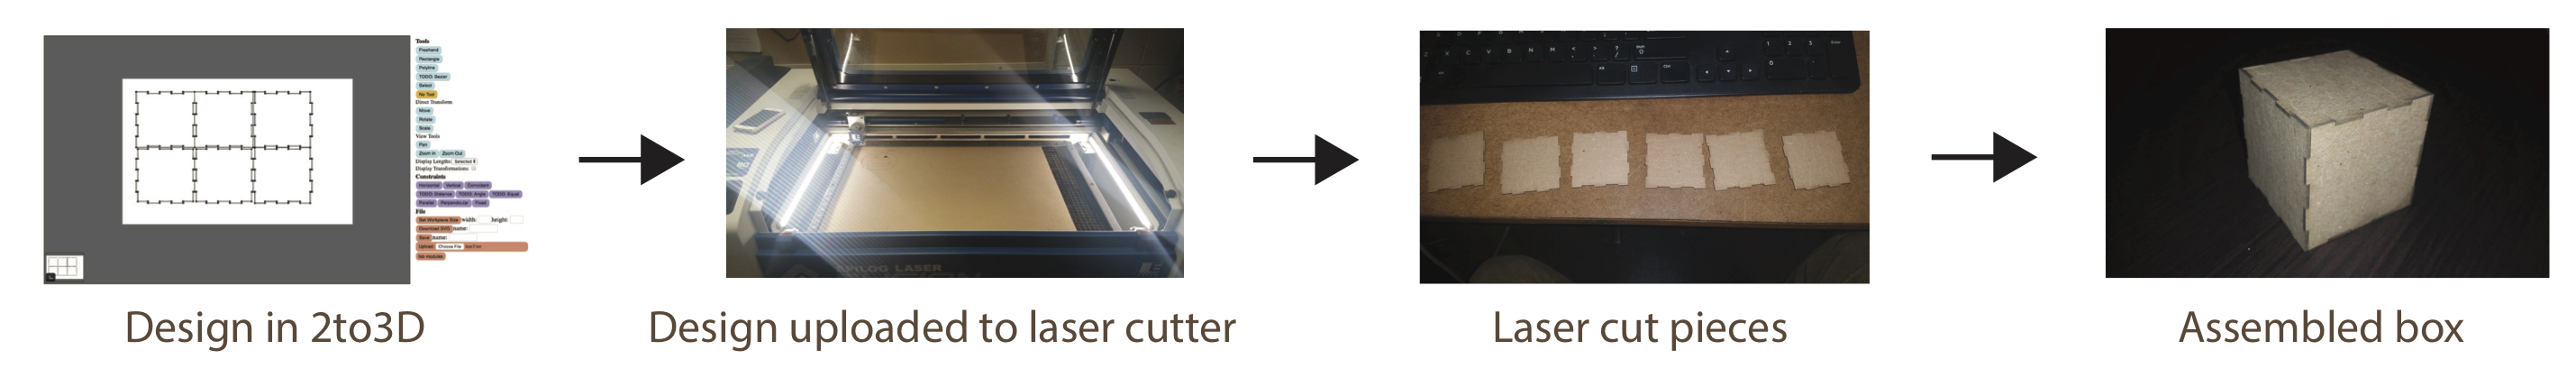
\includegraphics[width=\linewidth]{output}
  \caption{Full digital fabrication workflow using 2to3D. The laser cutter we had access to used CorelDraw for CAM so the drawing was created in 2to3D and imported to CorelDraw just for printing.}
  \label{fig:output}
\end{figure}

\begin{table}[]
\centering
\caption{Capabilities of 2to3D.}
\label{my-label}
\begin{tabular}{|l|l|l|l|}
\hline
\multicolumn{2}{|l|}{{\ul \textbf{Drawing}}}                                                                                                                                                        & \multicolumn{2}{l|}{{\ul \textbf{Navigation}}}                                                                                                                                               \\
\multicolumn{2}{|l|}{\begin{tabular}[c]{@{}l@{}}Freehand\\ Rectangle\\ Polyline\\ Bezier\end{tabular}}                                                                                              & \multicolumn{2}{l|}{\begin{tabular}[c]{@{}l@{}}Pan\\ Zoom in/out\end{tabular}}                                                                                                               \\ \hline
\multicolumn{2}{|l|}{{\ul \textbf{Direct Transformations}}}                                                                                                                                         & \multicolumn{2}{l|}{{\ul \textbf{Display Options}}}                                                                                                                                          \\
\multicolumn{2}{|l|}{\begin{tabular}[c]{@{}l@{}}Move\\ Rotate\\ Scale\end{tabular}}                                                                                                                 & \multicolumn{2}{l|}{\begin{tabular}[c]{@{}l@{}}Lengths\\ Transformation values\end{tabular}}                                                                                                 \\ \hline
\multicolumn{2}{|l|}{{\ul \textbf{Constraints}}}                                                                                                                                                    & \multicolumn{2}{l|}{{\ul \textbf{Other}}}                                                                                                                                                    \\
\multicolumn{2}{|l|}{\begin{tabular}[c]{@{}l@{}}Horizontal (line)\\ Vertical (line)\\ Coincident (points)\\ Fixed (points)\\ Parallel (lines)\\ Perpendicular (lines)\\ Length (line)\end{tabular}} & \multicolumn{2}{l|}{\begin{tabular}[c]{@{}l@{}}Click and drag points\\ Download SVG\\ Save drawing\\ Upload drawing\\ Copy/Paste\\ Delete\\ Hotkeys\\ Workarea size adjustable\end{tabular}} \\ \hline
\end{tabular}
\end{table}